
\section{Examples for the Export of Contributions}

The following sections contain content based on which an RDF document is constructed by RDFtex's preprocessor. The document is serialized and stored at \texttt{./exports.ttl}.

\subsection{Definition Export}

Here, we introduce the term \emph{noipper}. A noipper is the main technical component of a nopping machine. Its purpose is to nullify the interference that is caused by exceedingly high neipping values in the system.

\subsection{Dataset Export}

Of course, there is a multitude of available noippers from different brands. We compiled an exhaustive dataset that lists all available noippers and their features to allow for a fair comparison. The dataset is called noipperbase and is available at https://example.org/datasets/noipperbase.

\subsection{Experimental Result Export}

To ensure a safe operation, the noipper has to nullify the interference as fast as possible. We tested a readily available noipper in a typical neipping system and monitored the time it takes to nullify the interference when exceedingly high neipping values are encountered. On average, the process took 0.123 seconds based on 100000000 runs.  

\subsection{Figure Export}

\begin{figure}[htb!]
    \centering
    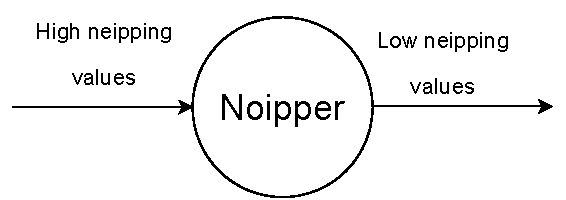
\includegraphics[width=0.8\columnwidth]{./figures/noipper_function}
    \caption{A diagram showing the function of a noipper.}
    \label{fig:scikg-structure}
\end{figure}

To illustrate the definition from above, \Cref{fig:scikg-structure} shows the function of a noipper.

\subsection{Software Export}

We also provide neippingviz, a tool for visualizing the neipping values of a system at \url{https://example.org/software/neippingviz-repo}. Upon startup, the neippingviz tool continuously monitors and displays fluctuations of neipping values in the system using appropriate diagrams. Wheneveer critical values are observed, warning messages are displayed. 

